
\documentclass[11pt,letterpaper]{article}
\usepackage{naaclhlt2010}
\usepackage{times}
\usepackage{latexsym}

\usepackage{amsmath}
\usepackage{amsfonts}
\usepackage{amssymb}
\usepackage{hyperref}
\usepackage{graphicx}
\usepackage{tikz}
\usepackage[justification=centering]{caption}
\usepackage{subcaption}
\usepackage[left=1in,right=1in,top=1in,bottom=1in]{geometry}

\usetikzlibrary{decorations.pathmorphing} % noisy shapes
\usetikzlibrary{fit}					% fitting shapes to coordinates
\usetikzlibrary{backgrounds}	% drawing the background after the foreground


\setlength\titlebox{6.5cm}    % Expanding the titlebox

\title{Handwritten Word Recognition using OCR and a Sequence Model}

\author{Daniel Deutsch\\
  Johns Hopkins University\\
  {\tt ddeutsch@jhu.edu}
  \And
  Daniel Crankshaw \\
  Johns Hopkins University \\
  {\tt dcrankshaw@jhu.edu}}

\date{}

\begin{document}
\maketitle

\section{Introduction}

A common problem in the field of machine learning is correctly identifying
handwritten numbers or words. The applications of
such a model are clear, and have already been implemented in situations like
the US postal service to sort mail based on the zip code.

We originally were going to look at individual numerical digit recognition using the famous
MNIST handwritten digit dataset, comparing the performance of K-Nearest-Neighbors and a
Neural Network. However, as we looked into it more we realized that this is essentially a solved
problem and not very interesting. Instead, we decided to try handwritten word recognition,
a more applicable and harder problem. We still wanted to compare the performance of multiple
models, and decided to stick with a Neural Network as one of the algorithms because it tends to
perform very well on optical character recognition tasks. Its \href{http://yann.lecun.com/exdb/mnist/index.html}{performance on the digit recognition benchmarks} reinforced our hypothesis that it would perform well on handwritten letter
recognition. Because we were now looking at whole words, we thought it would be interesting to take
into account the context of letters within a word when trying to identify them, taking advantage of
patterns of the English language. The natural model for this type of problem is a sequence model,
either a Hidden Markov Model or a Conditional Random Field. We decided to use an HMM after seeing
the success of Feng et al. \cite{feng} using a classifier with an HMM.

Our work compares how well two algorithms - a Neural Network and an Hidden Markov Model Neural
Network combination - perform on handwritten word recognition. The Artificial Neural Network (ANN) will
try to classify individual letters in a word based on their pixel values. The second algorithm will
use the ANN to classify individual letters as well, but will use the HMM to attempt to correct
misclassifications by looking at the probabilities of surrounding letter combinations and common
mistakes that the ANN makes. We hope that the addition of contextual information
about the surrounding letters will help improve the accuracy of the model.

\section{Related Work}

Feng et al.\ explores this idea of combining classification with a sequence
model in order to perform handwriting recognition on a large vocabulary corpus. They used a
joint-boosting algorithm to not only identify the letters, but perform letter segemenation. They
combined information about each individual letter with knowledge of the context of the letter in the
form of a supervised HMM.

Although the approach they take is more complicated, including the use of an ensemble of HMMs and
many more features, their success indicates that the combination of classification with an HMM is a
viable approach for the handwriting recognition problem.

\section{The Data and Algorithms}

{\bf Data:} The data that will be used in the training and evaluation of the ANN and the HMM was gathered from
\href{http://ai.stanford.edu/~btaskar/ocr/}{an optical character recognition dataset from
Stanford University}.
The data is a collection of handwritten letters segemented from words in which all uppercase
characters have been removed. We took the raw data and removed specific features included in the
data that we intended not to use. The resulting data set is a list of binary pixel values of each
character's 16 by 8 image.
\begin{figure}[h]
    \centering
    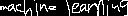
\includegraphics{img/ml.jpg}
    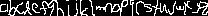
\includegraphics{img/alphabet.jpg}
    \caption{An example of the data set}
    \label{fig:exampleData}
\end{figure}

The data can often be difficult to read for a human as Figure~\ref{fig:exampleData} demonstrates.  Although it is
possible to make out each letter, this task is made much easier by looking at the context of the
word and anticipating what the letter should be. The figure also illustrates that many of the same
letters are a variety of different sizes and are placed at different locations within the image. The
quality of the data may make it difficult for the ANN to learn how to recognize each letter.
However, the combination of the ANN and the HMM may be a good simulation of how a human would
approach the problem: try to recognize the letter, then use context clues to figure out which
character it is.

The corpus used to learn the transmission probabilities for the HMM is a a Project Gutenberg
plain-text copy of \emph{Moby Dick}. We cleaned the corpus by converting all letters to lowercase
and removing all non-alphabetic characters (i.e.\ numbers and punctuation). Our training corpus is
the first half of the text and the test corpus is the second half of the text.

{\bf The Algorithms:} The two algorithms that we intend to use to accomplish the character recognition goal are an
artificial neural network (ANN) and a hidden markov model (HMM). The idea is to compare the accuracy
of the ANN to a combination of both the ANN and HMM to see if adding knowledge of word context to
the model increases accuracy on the datasets.

{\bf Neural Network Theory:} The original idea behind the artifical neural network was to simulate connections between neurons in
the brain. Each neuron receives a message, performs some type of computation, and sends a new
message to the neurons to which it is connected. For the artificial neural network, the intial input
is derived from the features of a data point. Based on this input, each neuron computes an
activation function (typically the sigmoid function) to see if it should be on or off. The new
values that are computed are multipled by a transition weight to the next layer of neurons. This
process repeates until the output layer has been reached. The values of each output neuron represent
a likelihood that the input data is of a specific class.

In order to train the algorithm, the backpropagation algorithm assigns specific error values to each
individual node, which creates the gradient function based on each of the parameters. With the
gradient function, an optimization algorithm like gradient descent can be use to find an optimum
value for each parameter. Neural networks are not convex, so there is no guarantee that the solution
is the global optimum.

\begin{figure}[h]
\centering
\caption{An example neural network}
\begin{tikzpicture}

\node (x1) at (0, 0) [draw,shape=circle]{};
\node (x2) at (0, 1) [draw,shape=circle]{};
\node (x3) at (0, 2) [draw,shape=circle]{};

\node (x4) at (1, 1.5) [draw,shape=circle]{};
\node (x5) at (1, 0.5) [draw,shape=circle]{};

\node (x6) at (2, 1.5) [draw,shape=circle]{};
\node (x7) at (2, 0.5) [draw,shape=circle]{};

\draw [->] (x1) -- (x4);
\draw [->] (x2) -- (x4);
\draw [->] (x3) -- (x4);

\draw [->] (x1) -- (x5);
\draw [->] (x2) -- (x5);
\draw [->] (x3) -- (x5);

\draw [->] (x4) -- (x6);
\draw [->] (x5) -- (x6);

\draw [->] (x4) -- (x7);
\draw [->] (x5) -- (x7);

\end{tikzpicture}
\label{fig:exampleANN}
\end{figure}

In Figure~\ref{fig:exampleANN}, each neuron is represented with a circle. Each weight parameter that is learned by the
backpropagation algorithm is shown by a line that connects the neurons in each layer.

{\bf Neural Network Implementation:} The ANN will be trained on the pixel values for each letter image. Each training example is a 16 by
8 pixel image which amounts to an input size of 128. In order to help improve the accuracy of the
classifier, we included a bias term on the input and hidden layers. Therefore, the input size for
the ANN is 129 nodes.

Similarly, since we are trying to classify each image as a letter, there will need to be 26 output
nodes, one for each lowercase letter in the alphabet. Therefore, the input and output sizes are set.
The only parameters left to tune for the ANN are the number of hidden layers and the number of nodes
within each hidden layer.

In order to find the best values for these parameters, we ran a series of tests on the development
data set to try and tune the parameters. We compared the accuracies of each model on the development
dataset to try and find the optimal parameters.

The following table was generated by randomly initializing an ANN with the given hidden layer sizes, then
training them all on the same data. This process is repeated 20 times per data point, and the
average accuracy is given. The accuracy is determined by if the classifier gets the data point
exactly correct. Another common metric is to test if it got the right answer within the top 5
guesses, but that is not used here.

For the ANN with one hidden layer, the only parameter than can be changed is the number of hidden nodes in that layer.

\begin{figure}[h]
    \caption{Accuracies of two-layer networks}
    \centering
    \begin{tabular}{|c|c|}
        \hline 
        Hidden Nodes & Accuracy \\ 
        \hline 
        25 & 54.86\% \\ 
        \hline 
        50 & 54.24\% \\ 
        \hline 
        75 & 52.13\% \\ 
        \hline 
    \end{tabular} 
\end{figure}

Since all three data points are relatively similar, and the smaller neural
network will train faster, we will use a network with one hidden layer and 25 nodes
in that layer.

This data is indicative of our belief that the neural network might have some
difficulty classifying this dataset. The input seems to be a relatively
difficult dataset with some noise. Since adding more nodes to the hidden layer
did not improve the accuracy significantly enough, it's evident that the
network is having a hard time learning the data. It may have reached its
maximal ability to learn. We hope that the combination of the HMM with the ANN
will help improve these accuracies.

One other idea that we tried was to add a second hidden layer to see if
increasing the number of weights allowed for improvement. With a small number
of tests, the amount of improvement was almost non-existent. Therefore, given
the extra amount of time it takes to train a neural network with two hidden
layers, we concluded that it was not worth the investment.

Therefore, the neural network that we will use in our experiments in
combination with and against the HMM will be a neural network with 128 input
nodes, 25 hidden nodes, and 26 output nodes, not counting the bias units.

Since it is possible to describe a neural network as a series of matrix multiplications, its
implementation will involve some non-trivial linear algebra functions. In order to do this
effectively in Java, we use the \href{http://math.nist.gov/javanumerics/jama/}{Java Matrix Package}.

In order to successfully implement the combined classifier, we separately
created an ANN and an HMM to independently perform their tasks. The ANN was
implemented with both a two and three-layer network structure. We tried to
find the optimal network structure to get the highest accuracy on the
recognition of the letters because we knew that it would be extremely important
for training the HMM\@. If the ANN was unsuccessful, then the HMM would not work
as well. After running several tests, the three-layer neural network did not
perform as well as the two-layer network. It is possible that this is due to
the algorithm being slightly more complicated to implement.

Once we had an accurate two-layer network implementation working, we varied the
hyperparameter which specificed the number of nodes in the hidden layer to see
if it affected the accuracy, which was previously discussed. Since altering the
size of the hidden layer did not significantly change the results, we
hypothesized that even a working three-layer network would not help to improve
the accuracy.

{\bf Hidden Markov Model Theory:} A Hidden Markov Model is a directed graphical model used for modeling sequences.
In general, modeling the probability of a given sequence is difficult because
the $n$th term in a sequence is dependent on all of the preceding terms. The key
insight in a Markov Model is that we can model most sequences very accurately
by looking at setting our current state dependent on only a fixed number of previous
states. If we look at the $k$ previous states, we get a $k$th order Markov chain.
A Hidden Markov Model extends this model to create a model such that an observation
is conditionally dependent on all previous observations, freeing us of the restrictive
assumption of a simple Markov chain. We introduce a set of latent nodes in an HMM such
that the hidden nodes form a Markov chain. This can be seen because any two latent nodes
$z_{n-1}$ and $z_{n+1}$ are independent conditioned on $z_n$. But there is always a path between any two
observed variables through the latent nodes which are never blocked and so the current
observed variables relies on all the previously observed variables \cite{bishop:607}.

\begin{figure}[htbp]
\centering
\tikzstyle{observed}=[circle, thick, minimum size=1.2cm, draw=red!80, fill=purple!25]
\tikzstyle{hidden}=[circle, thick, minimum size=1.2cm, draw=red!80]
\tikzstyle{background}=[rectangle,
                                                fill=gray!10,
                                                inner sep=0.2cm,
                                                rounded corners=5mm]

\begin{tikzpicture}[>=latex,text height=1.5ex,text depth=0.25ex]
    \matrix[row sep=0.5cm, column sep=0.5cm]{
        \node (z_1) [hidden]{$\mathbf{z}_{1}$};   &
        \node (x_1) [observed]{$\mathbf{x}_{1}$};   &
      \\
        \node (z_2)   [hidden]{$\mathbf{z}_2$};  &
        \node (x_2)   [observed]{$\mathbf{x}_2$};  &
      \\
        \node (dots) {$\cdots$}; &
                                 & %\node (bdots) {}; &
      \\
        \node (z_n-1)   [hidden]{$\mathbf{z}_{n-1}$};  &
        \node (x_n-1)   [observed]{$\mathbf{x}_{n-1}$};  &
      \\
        \node (z_n)   [hidden]{$\mathbf{z}_{n}$};  &
        \node (x_n)   [observed]{$\mathbf{x}_{n}$};  &
      \\
        \node (z_n+1)   [hidden]{$\mathbf{z}_{n+1}$};  &
        \node (x_n+1)   [observed]{$\mathbf{x}_{n+1}$};  &
      \\
    };
    \path[->]
    (z_1) edge (z_2)
    (z_2) edge (dots)
    (dots) edge (z_n-1)
    (z_n-1) edge (z_n)
    (z_n) edge (z_n+1)

    (z_1) edge (x_1)
    (z_2) edge (x_2)
    (z_n-1) edge (x_n-1)
    (z_n) edge (x_n)
    (z_n+1) edge (x_n+1)
    ;
    \begin{pgfonlayer}{background}
        \node [background,
                    fit=(z_1) (z_n+1) (x_1)] {};
    \end{pgfonlayer}


\end{tikzpicture}
\caption{The graphical structure of a hidden Markov model}
\end{figure}

There are three sets of parameters that must be learned in an HMM\@. The transition probabilities
$P(z | z_{n-1})$, which are the probabilities of transitioning from one hidden state to another,
the emission probabilities $P(x | z)$, which are the probabilities of observing a particular observed state
given the value of its corresponding latent variable, and the start probabilities $\pi$ which are the probalities
governing the state of the first latent node in the chain.

Many times a hidden Markov model does not have labeled data to train with, and must be trained using EM\@. In
this case, an algorithm known as the Forward-Backward algorithm - a special case of the Sum-Product algorithm -
can be used to efficiently perform the E-step of the algorithm. However, in our case we had labeled data
and so could directly learn these parameters.

Prediction with an HMM involves finding the most probable sequence of latent variables
that would result in the values found for the observed variables. We use the max-sum
algorithm, called the Viterbi algorithm in the context of hidden Markov models, to
find this sequence. The Viterbi algorithm is a dynamic programming algorithm that
for each state at each position in the sequence, only keeps track of the path leading
to that state with the highest probability. This means that we need only keep track of
$Z$ paths (where $Z$ is the number of possible states for a hidden node) at each position
in the sequence for a total of $Z N$ instead of the $Z^N$ total paths possible. The most
probable sequence can then be found by finding the value of the last hidden node that has
the highest probability path associated with it and then backtracking through the sequence
from there.


{\bf Hidden Markov Model Implementation:} Training the HMM is straightforward. There are three sets of parameters
that we needed to learn to make predictions. The first is the emission
probabilities for the ANN\@. 


We trained the HMM in a supervised setting, directly learning the parameters
from labeled data. We treat the actual letters that make up a word as the
hidden nodes ($z_i$) and the letters predicted by the ANN based on that
input as the observed nodes ($x_i$). The first set of parameters that the HMM
needs to learn are the emission probabilities $P(x_i | z_j)$. This is the probability
that the ANN predicts an observed letter $x_i$ given a letter representing
the state $z_j$. We learn these probabilities by testing the already
trained ANN on a set of labeled handwritten letter data (separate from the
data used to train the ANN), and counting the number of times the ANN predicted
each letter given a particular letter as input. We tested this with both a Bayesian
approach (by learning $P(z|x)$ as well as separately learning $P(x)$ and $P(z)$
from the training corpus) and a direct approach (learning $P(x|z)$ directly), and ultimately
decided on a the non-Bayesian method.

We then learned the transmission probabilities and the probability of each letter being the first
letter of a word by reading through the training corpus. We counted the number of times each
possible letter pair occurred and the number of times each letter was the first letter of a word and
divided by the total number of letter pairs and words respectively. We found through experimentation
that there were certain letter pairs that did not occur in training but did in testing, and so we
decided to add in Laplacian (+1) smoothing for the transmission probabilities.

For prediction, we implemented the Viterbi algorithm using two matrices, one to keep
track of the sequence probabilities at each position in the sequence and one to keep track
of the paths producing these sequences. Our implementation was based on the pseudocode
found in the \href{http://en.wikipedia.org/wiki/Viterbi_algorithm#Pseudocode}
{Wikipedia article} on the Viterbi algorithm.

\section{Results}

In order to compare the implementation and accuracy of the ANN versus the
HMM-ANN combination, we compared their performances with three different
metrics: the percentage of letters correct, the
percentage of fully correct words, and the average percentage of letters correct per word.

In the following figures, we compare the two algorithms with each of the three accuracy metrics. The
neural network was not retrained between tests. Its results were used to calculate the emission
probabilities for the HMM\@. The HMM, however, was retrained with four different subsets of the
training corpus: the first 12.5\% of the corpus, the first 25\%, the first 50\%, and then all of the
training data. Each algorithm was then tested on a random 10\% of the same test dataset, and the
results were averaged. This process was repeated on three subsets of words: small (2-4 letters),
medium (5-8 letters), and large (9+ letters) words.

\begin{figure}[h]
\centering
\caption{Percentage of letters correct}
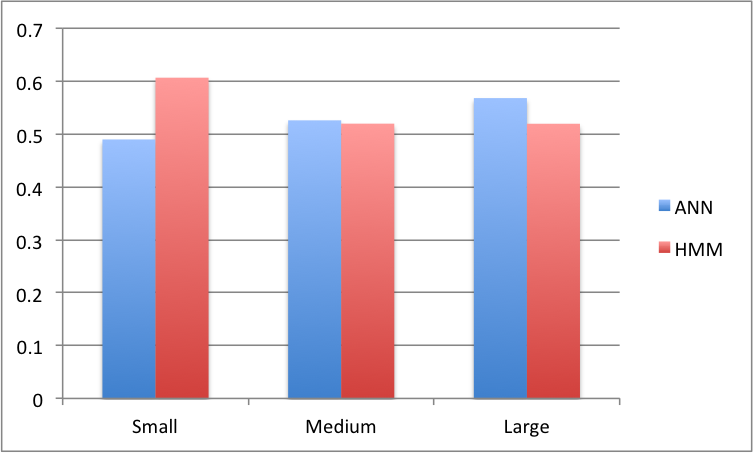
\includegraphics[scale=0.55]{img/lettersCorrect.png}
\label{fig:lettersCorrect}
\end{figure}

\begin{figure}[h]
\centering
\caption{Percentage of fully correct words}
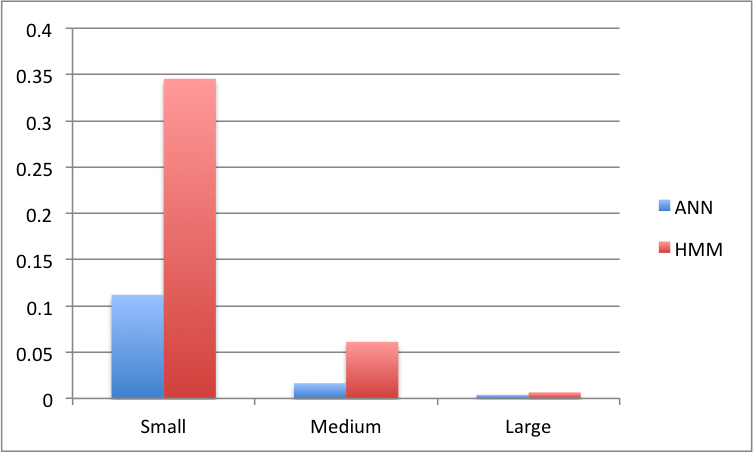
\includegraphics[scale=0.55]{img/wordsCorrect.png}
\label{fig:wordsCorrect}
\end{figure}

\begin{figure}[h]
\centering
\caption{Average percentage of letters correct per word}
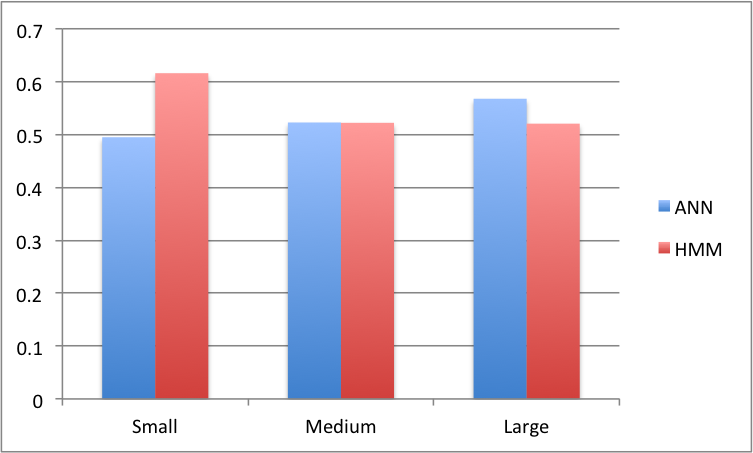
\includegraphics[scale=0.55]{img/wordCorrectness.png}
\label{fig:lettersCorrectPerWord}
\end{figure}

\section{Analysis}

We hypothesized that increasing the size of the training corpus would increase the accuracy of the
HMM because in order for the transmission probabilities to converge, we would need to look at a
certain amount of data. However, there was no significant difference in the HMM accuracy as we
changed the size of the training corpus. It is possible that even the smallest corpus was already
large enough for the transmission probabilites to have converged at approximately 14,000 words.

From Figures~\ref{fig:lettersCorrect} and~\ref{fig:lettersCorrectPerWord}, it is evident that as the length of the word increases, the accuracy of the
ANN-HMM combination decreases. We hypothesize that once the HMM begins to incorrectly identify a
sequence, it tends to continue to do so because of the weight of the transmission probabilities on
predicting the most probable sequence. In order to get a sequence back on the right track, we would
need a high correct emission probability and a high probability of transitioning from the previous
incorrect letter to the current correct letter, which effectively breaks the reasons behind using a
HMM\@. Because we use the same ANN-HMM combination on our short and long word predictions, we assume
the same probability of getting a starting down an incorrect subsequence at a given position in a
word regardless of the length of the word. Because the longer words have more positions at which to
start down a wrong sequence, and will tend to have more letters remaining in the word to be wrongly
predicted once an incorrect subsequence is started down, longer words will tend to have more
incorrect letters. However, this is still a hypothesis and we would need to run more
experiments to verify this. One possible experiment would be to create a frequency distribution of the letters for each of our word size buckets.

Let $f_{x,\alpha}=\frac{\textrm{occurrences of }\alpha}{\textrm{size of }x}$
where $\alpha$ is a letter, and $x$ is a word bucket size. Let $S_\alpha$ be
the accuracy of the ANN predicting $\alpha$ (see Figure~\ref{fig:letterAccuracies}). We can compute the
expected total accuracy of the ANN on each bucket by computing
\begin{equation}
E_x = \sum_{\alpha \in \{a,\ldots, z\}}f_{x,\alpha} s_\alpha
\end{equation}

If our hypothesis about longer words having higher frequencies of letters that the ANN does well on than shorter words, we would expect 
\begin{equation*}
E_{\textrm{small}} < E_{\textrm{medium}} < E_{\textrm{large}}
\end{equation*}


One interesting trend that we did not expect to see in the data is the slight increase in accuracy
of the ANN on the data set as the word length increases. This was surprising because the ANN
predicts each letter independently, so changing how the letters are grouped into words should not
have affected the accuracy. One potential explanation is that the ANN is much better at classifying
some letters than others. If the longer words tend to contain higher concentrations of those
``eaiser'' letters, then the ANN would have a higher accuracy on the larger word bucket. 

In order to investigate this further, we looked at the accuracy of the ANN on each specific letter.
As you can see from Figure~\ref{fig:letterAccuracies}, the results are highly variable, and there are even several letters
that have 0\% accuracy.

\begin{figure}[h]
\centering
\caption{Individual letter accuracies for the ANN}
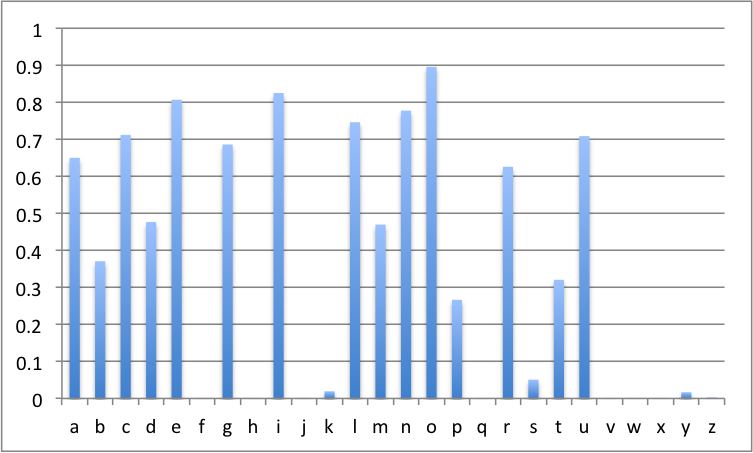
\includegraphics[scale=0.55]{img/letterPercentages.png}
\label{fig:letterAccuracies}
\end{figure} 

One potential reason for this high variability is that the number of training examples for the
different letters varies by an order of magnitude. The letters on which we did predicted very poorly
tend to occur less often in English, and therefore we did not have as many training examples for
those letters. This does not prove that the longer words contain less of the harder letters, but it
supports that it is a valid hypothesis. 

Additionally, the accuracy of the neural network even on those examples where
it performs well could still be improved. After analyzing the data a little bit
more to investigate if the noise could be a problem, we hypothesize that there
are a few reasons why the neural network has trouble learning to recognize each
letter. 

\begin{figure}[h]
\centering
\caption{Examples of the letters `a' and `e'}
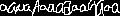
\includegraphics[scale=1.0]{img/aa.jpg}
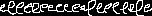
\includegraphics[scale=1.0]{img/ee.jpg}
\label{sampleLetters}
\end{figure}

Neural networks can be very slow and difficult to train. Sometimes, they
require a large amount of data in order to converge to a good solution, and it
helps if the data is somewhat normal. Figure~\ref{sampleLetters} demonstrates the variety that
each letter contains. The letters can often be small or large, they can be
located at the top of the image or the bottom, and even in some cases, the
capital version of the letter is used. These variations within the data can
pose a large problem for a neural network. It is asking a lot of the classifier
to be able to identy the letter `a' anywhere in the image whether it is capital
or not.

\section{Conclusion}

While our models did significantly better than random guessing, we still expected higher accuraices
that what we were able to obtain. It seems that the root of our issues with the HMM are directly
tied to the low accuracies of the neural network. We believe a lot of the issues with the neural
network were based on what turned out to be a very noisy and relatively sparse data set. 

One step in trying to improve the model would be to use less noisy data. We could perform optical
character recognition on typed letters instead of handwritten ones as this would minimize the amount
of variation between each letter.

Another option would be to add more features to the data set other than just the character's pixel
values. We could consult the computer vision literature to help with this additional feature
engineering.


\begin{thebibliography}{}

\bibitem[\protect\citename{{Bishop}}]{bishop:607}
\newblock Christopher M. Bishop.
\newblock 2006.
\newblock {\em Pattern Recognition and Machine Learning (Information Science and Statistics)}.
\newblock Springer-Verlag New York, Inc.

\bibitem[\protect\citename{Feng et al.}]{feng}
\newblock S. Feng, N. Howe, and R. Manmatha.
\newblock 2008.
\newblock {\em A hidden Markov model for alphabet-soup word recognition}.

\end{thebibliography}


\newpage
\appendix
\section{Interactive Classification}

We have provided an interactive classifier with a trained HMM and ANN\@. It allows the user
to type in a word or phrase. The program will then generate and display a picture of the handwritten
word from the letter data we used. It will then try to predict the word and display the model's
prediction below the user's input.

The program can be run from within the \texttt{interactive-recognizer}
directory with the following commmand:\\\\
\texttt{\$ java -jar InteractiveRecognizer.jar}

\section{Comparison to Proposal}
We ended up changing our project substantially after receiving feedback on our original proposal. We
met with Professor Dredze to dicuss our new project and were not required to submit an entire new
proposal. Therefore, we don't really have an applicable proposal to compare the our progress to.
However, we do discuss the evolution of our project from the proposal to its current form
in our introduction.


\end{document}
